\section{Nation-State Routing: Default \\Routes}
\label{measure}

\newcommand{\headrow}[1]{\multicolumn{1}{c}{\adjustbox{angle=45,lap=\width-0.5em}{#1}}}
\newcolumntype{P}[1]{>{\raggedright\arraybackslash}p{#1}}
\begin{table*}[t]
\centering
\begin{tabular}{|P{37mm}|cc|cc|cc|cc|cc|}
\multicolumn{1}{l}{}    & \headrow{Host} & \headrow{Transit} & \headrow{Host} & \headrow{Transit} &\headrow{Host} &\headrow{Transit} &\headrow{Host}   &\headrow{Transit} &\headrow{Host}  &\headrow{Transit} \\\hline
\textit{Country}    &\multicolumn{2}{c|}{\textit{Brazil}}   &\multicolumn{2}{c|}{\textit{Netherlands}}   &\multicolumn{2}{c|}{\textit{India}} &\multicolumn{2}{c|}{\textit{Kenya}} &\multicolumn{2}{c|}{\textit{United States}}\\
\hline\hline
Brazil             &.169     &1.00   &     &  &   &   &    &     &  & \\\hline
Canada             &.001     &.013   &.007     &.007  &.015    &.016   &.006    &.008     &  &.081 \\\hline
France             &.001     &.059   &.022     &.102  &.009    &.104   &.023    &.221     &.0013  &.104 \\\hline
Germany             &.002     &.005   &.013     &.050  &.014    &.032   &.028    &.048     &.0013  &.008 \\\hline
Great Britain             &.00006     &.024   &.019     &.140  &.021    &.204   &.032    &.500     &.0024  &.006 \\\hline
India             &    &   &     &.0007  &.053   &1.0   &.002    &.058     &  &.0005 \\\hline
Ireland             &.016     &.028   &.064     &.106  &.027    &.031   &.108    &.133     &.0012  &.006 \\\hline
Kenya             &    &   &     &  &   &   &.022    &1.0     &  & \\\hline
Mauritius             &     &   &     &  &    &   &.004    &.322     &  & \\\hline
Netherlands             &.013     &.019   &.392     &1.0  &.101    &.121   &.200    &.253     &.024  &.031 \\\hline
Singapore             &    &.0009   &.002     &.002  &.103    &.270   &.027    &.040     &  &.003 \\\hline
South Africa             &    &   &     &  &   &   &.021    &.334     &  & \\\hline
Spain             &.001     &.176   &    &.004  &   &   &   &     &  & \\\hline
United Arab Emirates             &     &.00003   &     &  &   &   &.011    &.152     &  & \\\hline
United States             &.774     &.844   &.454     &.583  &.629    &.715   &.443    &.616     &.969  &1.0 \\\hline
\end{tabular}
\caption{Fraction of paths that each country sees in default routes.}
\label{tab:transit_host}
\end{table*}

As Internet traffic crosses international borders, it becomes subject to the wiretapping policies of the national jurisdiction in which it is transitting.  We study five different countries, Brazil, Netherlands, India, Kenya, and the United States, and measure which countries are transitting their traffic.  The methods we use are described in Section \ref{pipeline1}, and in this section we discuss our findings.

\subsection{Hosting Diversity}
First we look at hosting diversity.  This shows us how many unique countries in which a domain is hosted -- the more countries that a domain is hosted in creates a greater chance that the content is replicated in a favorable country, and could potentially allow a client to circumvent an unfavorable country.  By querying DNS from 26 vantage points around the world, we found that there is hosting diversity among the Alexa Top 100 Domains.  About half of the Alexa Top 100 Domains in each of the five countries studied are hosted in more than one country.  This can be seen in Figure~\ref{fig:host_diversity}.  The amount of hosting diversity motivates the potential for circumventing surveillance states.  We next look at which countries are currently transitting and hosting Internet traffic, and measure whether traffic is going to replicas in surveillance states (when they may not need to).

\begin{figure}
\centering
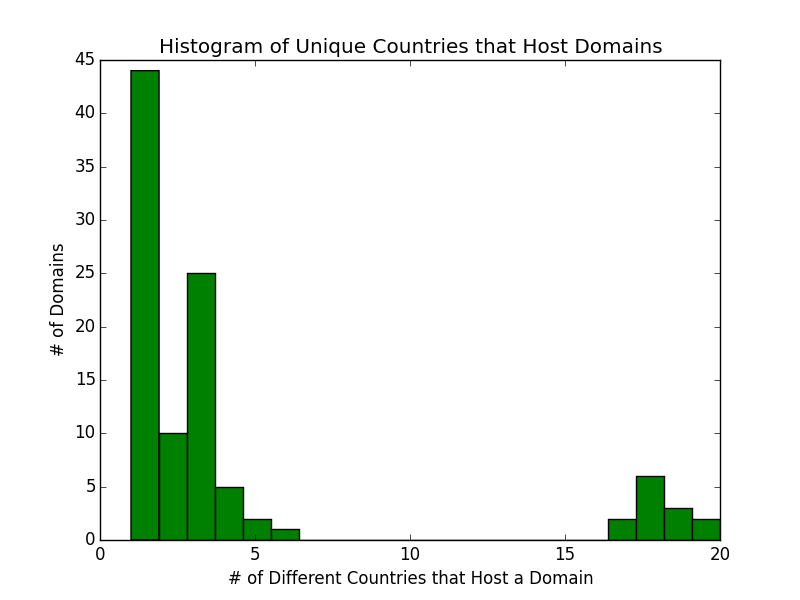
\includegraphics[width=.5\textwidth]{host_domains_hist_US}
\caption{The number of Alexa Top 100 US Domains hosted in different countries.}
\label{fig:host_diversity}
\end{figure}

\subsection{Trend 1: Surveillance States Host Domains}
\label{trend1}
Despite the amount of country-level hosting diversity, we see the majority of paths from all five countries ending in a single country.  The fraction of paths that are hosted in various countries can be seen in Table~\ref{tab:transit_host}.  The most common destination among all five countries studied is the United States: 77\%, 45\%, 63\%, 44\%, and 97\% of paths originating in Brazil, Netherlands, India, Kenya and the United States, respectively, are currently reaching content located in the United States.  This is significant because the United States is a known surveillance state, and therefore these percentages represent just a portion of foreign traffic that the United States can conduct surveillance on.  Our results also show the Netherlands as a common hosting location for traffic originating in the Netherlands, India, and Kenya.

For Indian traffic, in addition to the 63\% hosted in the United States and the 10\% hosted in the Netherlands, another 10\% is hosted in Singapore.  This can best be explained by the number of underwater cables with landing points in both India and Singapore~\cite{cablemap}.  More specifically, there is a cable that directly connects Chennai, India and Changi North, Singapore, and is owned by Tata Communications, which is one of the top global Internet providers (in terms of transitted IP space)~\cite{bakers}.  

For Kenyan traffic, the United States hosts 44\% of the content, but Ireland hosts 10\%; Ireland is a popular hosting location for U.S. companies due to it's relaxed enforcement of privacy in the private sector.  

It is also worth noting that most of the countries studied host a small percentage of their own traffic.  For traffic that originates in Brazil, only 17\% of it also ends in Brazil.  Only 5\% and 2\% of Indian and Kenyan traffic, respectively, end in the originating country.  In addition, only a fraction of country code top-level domains are hosted with in the respective country.  For Kenya, 24 of the Top 100 Domains are .ke domains, and of these 24 domains only 5 are hosted within Kenya.  29 out of 40 .nl domains are hosted in the Netherlands; 4 of 13 .in domains are hosted in India; 18 of 39 .br domains are hosted in Brazil.  Interestingly, all .gov domains were hosted in their respective country.

\subsection{Trend 2: Traffic Transits Surveillance States}
Similar to the trend of hosting domains, the United States also transits a large portion of foreign traffic -- it transits a larger portion of traffic than it hosts.  Brazilian traffic traverse the United States on 84\% of the paths; therefore, the United States can conduct surveillance on 84\% of the traffic originating in Brazil, despite Brazil's strong efforts in avoiding United States surveillance.  Even though India and Kenya are geographically distant, 72\% and 62\% of their traffic transits the United States.  Of the five countries studied, the Netherlands has the lowest percentage of traffic that transits the United States at 58\%.  

Great Britain and the Netherlands are on the path for a significant percentage of traffic originating in India and Kenya.  50\% and 20\% of paths that originate in Kenya and India transit Great Britain.  Traffic that traverses the Netherlands can be explained by the large IXP located there; traffic that traverses Great Britain is likely due to being on the path between the originating country and the final destination in a European country.

Mauritius, South Africa, and the United Arab Emirates transit 32\%, 33\%, and 15\% of traffic from Kenya.  There are direct underwater cables from Kenya to Mauritius, and from Mauritius to South Africa.  Additionally, there is a cable from Mombasa, Kenya to Fujairah, United Arab Emirates.  This accounts for the large percentages of traffic that pass through these countries.

\subsection{Trend 3: Tromboning Traffic Transits Surveillance States}

As mentioned in Section \ref{trend1}, the percentage of domestic traffic in some of the countries studied is extremely small.  For India, only 5\% of traffic is domestic and for Kenya, 2\% is domestic; despite the small amount of domestic traffic, some of this traffic trombones.  This can be seen better in the cases of Brazil and the Netherlands; figure \ref{trombone_netherlands} shows the amount of paths that trombone to differing countries for the Netherlands.

\begin{figure}
\centering
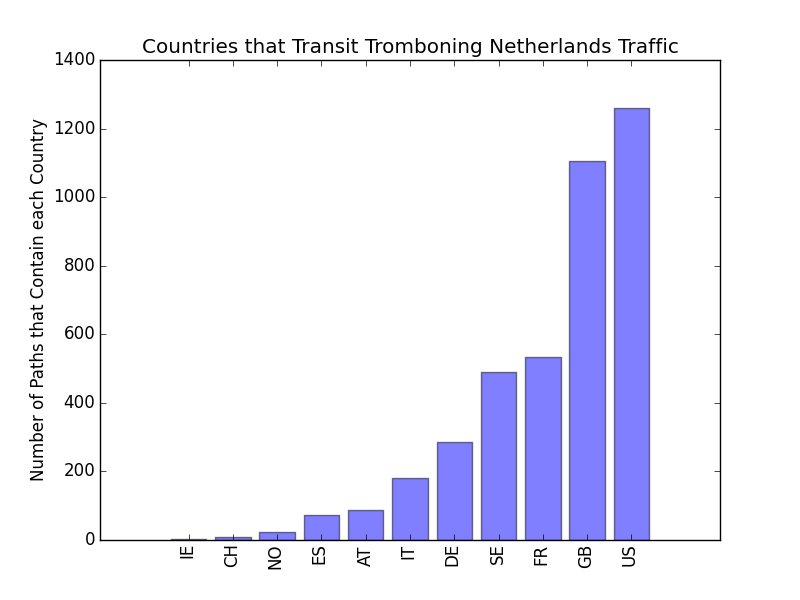
\includegraphics[width=.5\textwidth]{nl_trombone_no_none2}
\caption{The countries that tromboning Netherlands traffic transits.}
\label{fig:trombone_netherlands}
\end{figure}

24\% of all paths originating in the Netherlands (62\% of domestic traffic) trombone to a foreign country before returning to the Netherlands; The most common countries traffic trombones to are the United States and Great Britain.  Traffic that should be kept local is susceptible to surveillance because it transits two well-known surveillance states.  For Brazil, 5\% of all traffic starts in the Netherlands, transits a foreign country, and returns to the Netherlands (30\% of domestic traffic trombones).  The most common country traffic trombones to is the United States. 

\subsection{United States as an Outlier}

Most of the results discussed thus far have shown that Brazilian, Netherlands, Indian, and Kenyan traffic often transit surveillance states, most notable the United States.  The results from studying traffic that originates in the United States are drastically different from those of the other four countries.  The other four countries hosted very small amounts of their own traffic, whereas the United States hosts 97\% of the content that is accessed from witin the country.  Only 13 unique countries are ever on a path from the United States to a domain in the Top 100 (or third party domain), whereas 30, 30, 25, and 38 unique countries are seen on the paths originating in Brazil, Netherlands, India, and Kenya.  There are only 6 foreign countries that host content for traffic originating in the United States, and the fraction of content hosted in these countries is less than 4\% combined.
